\documentclass[ebook,12pt,oneside,openany]{memoir}
\usepackage[utf8x]{inputenc}
\usepackage[bulgarian]{babel}
\usepackage{url}
\usepackage{lipsum}
% Според изискванията на ИИКТ-БАН не бива да има номерация на страниците в ръкописа.
\usepackage{nopageno}
\usepackage{shorttoc}
\usepackage{graphicx}
\usepackage{imakeidx}

% Заглавие на книгата.
\title{Научни изчисления с Java и Android}

% Имена на авторите.
\author{Тодор Балабанов, Илиян Занкински, Петър Томов}

% Автоматично създаване на азбучен указател.
\makeindex[columns=1, title=Азбучен указател, intoc]

\begin{document}

\maketitle

% Заглавната страница не е с оформлението на останалата част от документа (няма номерация).
\thispagestyle{empty}

% Тук стои таблицата със съдържанието, което се генерира от названието на главите.
\newpage
\shorttoc{Теми}{0}

% Тук стои таблицата със съдържанието, което се генерира от названието на главите и названието на секциите в тях.
\newpage
\tableofcontents

% По този начин номерацията на подточките е с арабски цифри.
\renewcommand\thesection{\thechapter.\arabic{section}}
\renewcommand\thesubsection{\thesection.\arabic{subsection}}

\newpage
\addcontentsline{toc}{chapter}{Предговор}
\chapter*{Предговор}

Това учебно помагало е предназначено за ученици и студенти, които биха искали да се запознаят с възможностите за реализиране на \index{изчисления в разпределена среда} с използването на програмния език Java и мобилната платформа Android.

В съвременното ни ежедневие ние все по-често сме заобиколени от мобилни изчислителни устройства. Най-често това са мобилни телефони, таблети, часовници или други форми на wearables (миниатюрна електроника под формата на модни аксесоари или части от дрехи). До преди десетилетие този вид мобилни устройства бяха рядкост, а изчислителните им възможности бяха изключително ограничени. Тези два факта не позволяваха мобилните устройства да бъдат използвани за нещо повече освен основния принцип на употреба за който са създадени. С развитието на микроелектрониката и миниатюризацията на компонентите съставящи мобилните устройства техните възможности значително нараснаха за последното десетилетие. Това позволява върху този вид устройства да се извършват и допълнителни задачи, които не са били предвидени при първоначалното им проектиране. Паралелно с развитието на мобилните технологии бурен подем претърпяха и възможностите за мобилна комуникация като GSM, 3G, 4G, Wi-Fi, Bluetooth, NFC и други. Комбинацията между относително мощни мобилни изчислителни устройства и добре развита комуникационна среда открива безгранични възможности за приложение на мобилните устройства при извършването на допълнителни изчисления, в разпределена среда. 

В настоящето учебно помагало ще запознаем читателите с интересните възможности, които предлагат съвременните Android \index{мобилни устройства}, за постигането на резултати в научни изчислителни задачи, разпределяйки изчисленията върху физически отдалечени едно от друго устройства. 

\newpage
\chapter{Научни изчисления}

Още в зората на съвременната изчислителна техника най-съществените пресмятания са били с научна насоченост и военно дело. Този факт не се е променил значително за последните десетилетия. Дори в наши дни най-сериозните изчислителни ресурси са насочени в областта на науката. Това дава основание да обърнем значително внимание на начините по които можем да изпълняваме научни изчисления дори и върху изчислителни устройства, чието основно предназначение не е с научна цел. 

\section{Последователно програмиране}

При \index{последователното програмиране} всяка изчислителна инструкция следва всички предходни. В зората на изчислителната техника пресмятанията са извършвани по този начин. Дори в наши дни значителна част от алгоритмите се изпълняват само последователно, тъй като входните данни за всяка инструкция зависят от изходните данни на предходните инструкции. Последователните алгоритми не подлежат на декомпозиране и поради тази причина са неприложими за паралелни пресмятания. 

\begin{figure}[h!]
  \centering
  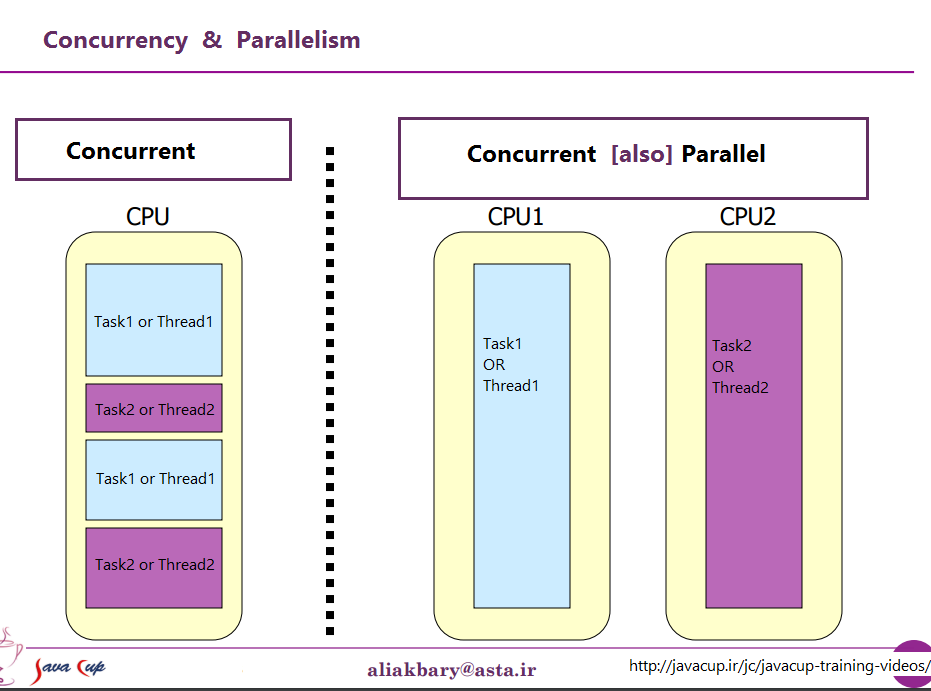
\includegraphics[width=1.0\linewidth]{./images/pic0002.png}
  \caption{Сравнение между последователни пресмятания и паралелни пресмятания.}
\label{fig:pic0002}
\end{figure}

\section{Паралелно програмиране}

При паралелното програмиране основно се говоир за две разновидности - \index{конкурентни пресмятания} и \index{паралелни пресмятания}. Конкурентните пресмятания са в среда където група от задачи могат да се пресметнат едновременно, без да има значение от реда на пресмятане. В същото време, паралелните пресмятания се отнасят за едновременно пресмятане на отделни задачи, върху отделни процесори. В този контекст всички паралелни пресмятания са конкурентни пресмятания, но не и обратното (Фиг. \ref{fig:pic0001}). 

\begin{figure}[h!]
  \centering
  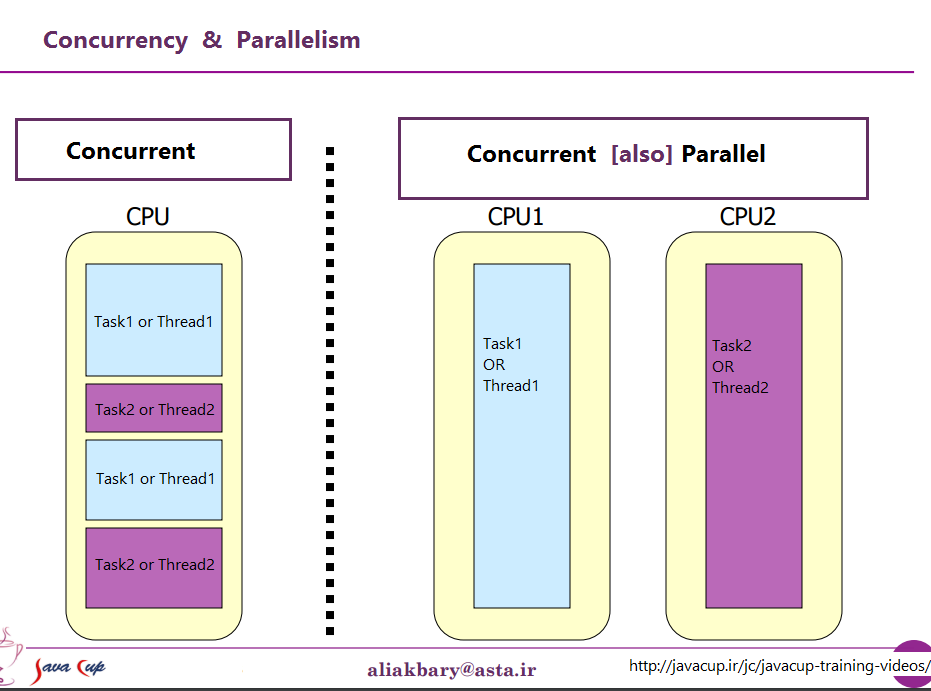
\includegraphics[width=1.0\linewidth]{./images/pic0001.png}
  \caption{Сравнение между конкуретни пресмятания и паралелни пресмятания.}
\label{fig:pic0001}
\end{figure}

\section{Супер компютри и грид изчисления}

Когато паралелните алгоритми се изпълняват на изчислителни машини с множество процесори и/или множество ядра на процесорите, този вид изчисления се определят като супер компютърни (supercomputing). Същественото при този вид пресмятания е, че се използва много бърз вътрешна шина (понякога оптична) и споделена оперативна памет. За разлика от \index{супер компютрите} \index{грид изчисленията} се осъществяват на множество машини, свързани в обща мрежа, но работещи автономно, без да споделят обща памет. При грид системите отделните изчислителни машини могат да са териториално отдалечени една от друга. Съществено е да се отбележи, че и при супер компютрите собственикът на системата има пълен контрол над нея. Това може малко да се различава за грид системите, ако към грида са включени компютри под чужд контрол. 

\section{Изчисления в разпределена среда}

\section{Дарена изчислителна мощност}

\newpage
\addcontentsline{toc}{chapter}{Заключение}
\chapter*{Заключение}

Основна цел на настоящото учебно помагало бе представянето на възможностите, които съвременните Android мобилни устройства могат да предложат за извършване на научни изчисления в разпределена среда. Без да претендира за изчерпателност изложеният материал има за цел да провокира творческото мислене у читателя и да го вдъхнови за създаването на собствени авторски проекти с разгледаните технологии и засегнатите научни области.  

Авторите са благодарни на своите читатели за отделеното време и внимание, като горещо насърчават подаването на обратна връзка и споделянето на интересни мисли, идеи или предложения, на посочените за връзка контакти.

% Списък с използвана литература и източници на информация.
\newpage
\begin{thebibliography}{99}
\end{thebibliography}

% Азбучен указател на използваните термини.
\newpage
\printindex

\end{document}